% !TeX spellcheck = fr_FR
\chapter{La distance et le temps}\label{ch:distancetemps}

De même que pour tout art martial, le temps et la distance sont des notions essentielles en escrime.
Ce n'est que par leur maîtrise que l'on peut vraiment espérer devenir une fine lame.

Intimement imbriqués, ces deux concepts ne sont toutefois pas des notions absolues et fixes ni des dimensions physiques réelles.
Tout en étant d'une aide incontestable pour décrire et commenter objectivement les actions d'escrime, ils recouvrent le sens du temps et de la distance dans un contexte de confrontation, c'est-à-dire la perception que peuvent avoir les adversaires de leurs capacités d'action relatives.
En tant que tels, le temps et la distance sont au c\oe{}ur des tactiques et de la stratégie de l'escrime.

\section{Temps d'escrime} \index{temps d'escrime}
Le \emph{temps d'escrime} est une unité de temps définie comme la durée d'une action simple : un pas, une coupe, un estoc, une parade, etc. \index{actions simples}
Le nombre d'unités de temps que dure une action combinée est le nombre d'actions simples consécutives qui la composent, des actions simples simultanées ne comptant que pour une unité de temps.
Par exemple, deux temps sont nécessaires pour parer en passant puis riposter.

Le temps d'escrime ne correspond pas strictement au temps d'horloge, il ne s'agit pas d'une durée définie puisqu'une action simple durera plus ou moins longtemps selon la vitesse à laquelle elle est exécutée.
Le temps d'escrime est plutôt lié à la notion d'engagement dans une action sous-tendue par une intention. \index{intention} 
Tant que le bretteur ne s'est pas totalement engagé dans son action, il peut transformer \index{transformation} et modifier son intention durant la même unité de temps.
Ce n'est qu'après engagement total qu'il devient impossible d'interrompre le cours de l'action et de changer d'intention pendant le même temps d'escrime.
Ceci ne signifie toutefois pas qu'une action doit être nécessairement menée à son terme dès qu'elle a été engagée mais seulement que les transformations prennent plus de temps lorsque l'intention est totalement exprimée.

Cette notion tactique primordiale est utilisée dans les feintes et fausses attaques.
Comme nous le verrons plus loin, lors d'une feinte, on ne s'engage pas totalement dans l'action offensive mais celle-ci doit être suffisamment convaincante pour forcer l'adversaire à s'impliquer totalement dans la parade de ce qu'il croit être une attaque. 
Il est alors possible de modifier l'action initiale dans le même temps et lancer la véritable attaque alors que l'adversaire est tout occupé à sa réaction initiale.
En règle générale, il est préférable d'éviter de s'engager trop tôt dans une action de manière à préserver aussi longtemps que possible la capacité de transformer et de s'adapter efficacement aux réactions de l'adversaire.

Le temps d'escrime est donc une notion théorique permettant d'évaluer la capacité d'initiative, de transformation ou de réponse des bretteurs durant les différentes actions.
On peut ainsi formaliser le cours des actions simples pendant l'étude d'une \emph{phrase d'arme}, quelle que soit la vitesse à laquelle elle est réalisée et en supposant que les deux adversaires sont aussi rapides l'un que l'autre.
Bien entendu, en réalité, certains escrimeurs sont plus rapides que d'autres mais en vérité, la vitesse n'a aucune importance. Seul le tempo compte vraiment : l'action juste au bon moment.  
Il est toujours possible de compenser une moindre vitesse par la mise en \oe{}uvre efficace de techniques et tactiques et, par-dessus tout, par la maîtrise du rythme.\index{rythme}
Un bretteur plus rapide peut perdre son avantage s'il est forcé par un adversaire plus compétent d'utiliser plus de temps d'escrime pour ses actions. 
Cette stratégie est parfois utilisée par certains escrimeurs qui, tout en prenant leur temps, n'ont de cesse de maintenir leur adversaire dans une situation d'urgence permanente.
Qu'ils le fassent en maintenant leur adversaire sous la menace constante d'une touche ou en sortant systématiquement de ses lignes d'attaque, ils imposent leur rythme et ne laissent pas leur adversaire reprendre l'initiative.
Pour atteindre ce but, il leur est toutefois indispensable de rester connecté à leur adversaire et que leurs mouvements et les menaces qu'ils lui font soient parfaitement adaptées à ses réactions.
En d'autres termes, le rythme du combat est en réalité une combinaison des rythmes des deux adversaires.
Bien que le rythme d'un escrimeur puisse dominer celui de l'autre, il y a toujours interdépendance : il est essentiel d'être connectés et reliés en permanence.

La capacité à comprendre et suivre le rythme de l'adversaire tout en dissimulant le sien propre est donc fondamentale pour pouvoir saisir l'instant juste et prendre l'avantage.
Il est essentiel de rester en permanence à l'écoute des mouvements de l'adversaire et de ne pas se laisser entraîner dans une anticipation inconsidérée par une régularité trompeuse du rythme.
Une attention toute particulière devrait également être portée à ne pas adopter un rythme trop régulier qui serait par conséquent facilement prévisible par l'adversaire.
Contrôler le rythme implique un état d'esprit relâché nous assurant d'être constamment prêt à nous adapter à la situation et à la transformer à notre avantage en répondant aux actions de l'adversaire de manière imprévisible.
Cependant, bien plus que d'avoir des réactions rapides  \textemdash{} vitesse n'est pas précipitation \textemdash{} il s'agit assurément de se tenir sur le fil d'un perpétuel présent, lâchant le passé et accueillant le futur sans s'attacher à aucune technique préconçue.

\section{Distance et mesure}\index{distance}
De même que le temps d'escrime ne représente pas une durée objective, l'effet de la distance entre les deux adversaires sur leur capacité relative à s'atteindre mutuellement est ici plus importante que leur distance physique réelle.
On définit ainsi la mesure \index{mesure} comme la distance en deçà de laquelle il est possible d'atteindre l'adversaire en un temps d'escrime.
En d'autres termes, c'est une distance suffisamment courte pour ne pas nécessiter plus d'un pas pour toucher.
Si au moins deux pas sont nécessaires, on est dit hors mesure.

On peut, à partir de là, définir trois distances en mesure :
\begin{enumerate}
\item \emph{Distance de garde} ou \emph{mesure longue} : 
un pas est nécessaire pour toucher. Cette distance offrant un bon compromis entre une attitude prudente et une tendance plus agressive, c'est une distance fréquemment adoptée pendant un assaut libre.
\item \emph{Distance de touche} ou \emph{mesure courte} : 
à cette distance, il est possible de frapper avec la partie appropriée de la lame sans avoir à faire un pas ni vers l'avant ni vers l'arrière.
\item \emph{Distance rapprochée}: 
cette distance est trop courte pour permettre une utilisation efficace de la lame, seules les techniques de corps à corps sont utilisables : coups de pied, de poing, saisies, etc. 
\end{enumerate}

Mais la mesure est plus qu'une distance.
Elle est influencée en effet par les postures des escrimeurs et leurs angles d'attaque respectifs.
La garde et la position des pieds détermine la portée maximale de l'épée atteignable en un temps d'escrime par une action simple : pas, transfert de poids, rotation du bras et du corps.\index{actions simples}
L'angle d'attaque et la manière dont l'adversaire se couvre sont les facteurs principaux déterminant si la cible pourra alors être atteinte par une coupe ou un estoc efficace.

Il faut garder à l'esprit que l'angle d'attaque comme la portée de l'épée ne doivent pas être uniquement considérés dans le plan horizontal mais en trois dimensions.
Ainsi, en toute situation, les cibles les plus proches sont celles approximativement situées à hauteur d'épaule, c'est-à-dire, la plupart du temps, le haut de la poitrine et la gorge.
Il est possible d'atteindre les cibles plus basses en avançant, mais aussi en s'accroupissant ou en se penchant de manière à abaisser l'épaule en face de la cible.

La figure \ref{fig:distance_stance} montre l'effet de la posture, des déplacements et de la hauteur de la cible sur la portée de l'épée.

\begin{figure}[ht]
\centering
	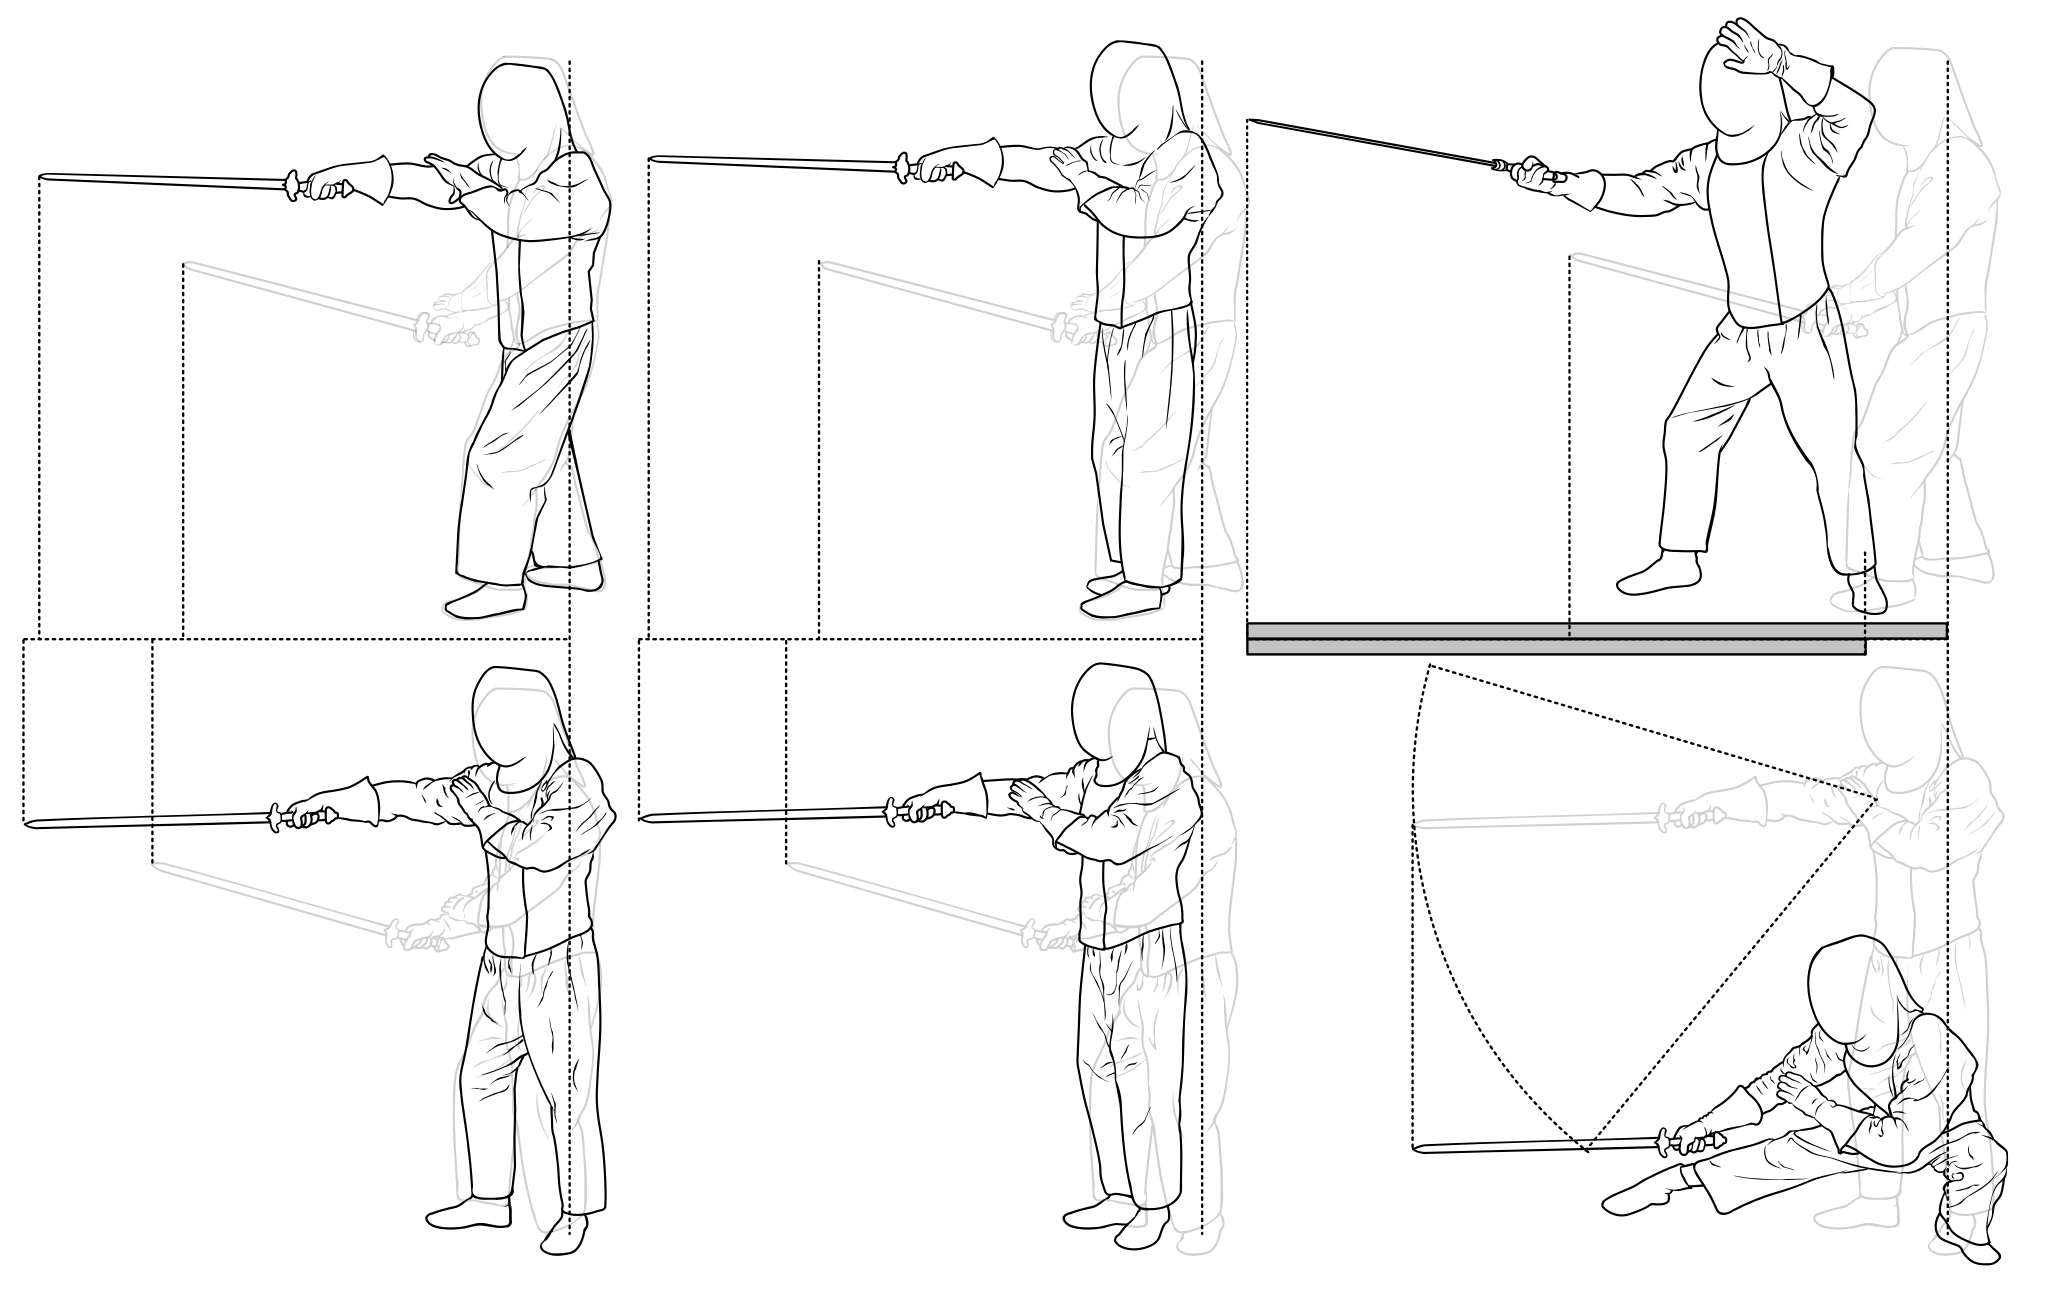
\includegraphics[width=1.0\textwidth]{../../Images/DistanceTime/distance_stance.pdf}
	\caption[Posture et mesure]{Quelques exemples de postures et leur portée en estoc. 
	
	La colonne de gauche montre la distance atteinte par l'extension du bras à partir de la position de garde initiale (représentée en gris). Cette distance est légèrement plus longue avec le pied droit en avant (figure du bas) grâce à la plus grande amplitude de rotation du corps poussant l'épée plus en avant. On peut faire une observation similaire sur la position de garde qui s'étend légèrement plus en avant avec le pied droit devant. La même remarque s'applique à la colonne du milieu montrant la distance atteinte en étendant le bras et en serrant le pas. La différence est toutefois moindre ici en raison d'une distance plus courte entre les pieds.
	
	La figure en haut à droite montre la portée maximale d'un estoc. Ainsi, le rectangle gris supérieur représente la longueur de la mesure en partant le pied gauche en avant. Grâce au déplacement de l'axe sur le pied gauche et à la passe avant, cette mesure est plus longue qu'en partant directement avec le pied droit devant.
		
	Sur la figure en bas à droite, l'arc de cercle représente la portée verticale de l'épée en se tenant debout sans faire de pas. Bien qu'elles puissent ne pas être horizontalement plus loin de l'axe du corps, les cibles basses n'en sont pas moins hors d'atteinte à moins de s'accroupir de façon à amener l'épaule à leur hauteur.
	
	Toutes  les figures sont représentées à la même échelle.}
	\label{fig:distance_stance}
\end{figure}

La nature dynamique de l'escrime requiert de surcroît d'examiner la notion de mesure dans un contexte mouvant, changeant avec le moindre mouvement des adversaires.
Étant donné que s'éloigner de la cible augmente la distance, il est possible d'être suffisamment près pour être en mesure statiquement tout en étant en même temps dynamiquement hors mesure.  
Temps et distance se combinent et la durée relative du temps d'escrime pour chacun des deux adversaires diminue ou s'allonge selon que leurs pas les rapprochent ou les éloignent de leur cible.
%
%\begin{figure}[ht]
%\centering
%	\includegraphics[width=0.69\textwidth]{../../Images/EmptyFig.pdf}
%	\caption[Déplacement et mesure]{Déplacement et mesure}
%	\label{fig:distance_motion}
%\end{figure}

Le concept de mesure n'est en effet pas symétrique et les adversaires ne sont pas nécessairement à la même mesure l'un relativement à l'autre en raison de postures différentes, de leurs déplacements relatifs et de leurs angles d'attaque respectifs. 
\FloatBarrier
%Comme le montre la figure \ref{fig:distance_motion},
On peut donc tirer avantage de ce caractère asymétrique en se déplaçant vers une direction et avec un angle permettant de rester en mesure tout en empêchant l'adversaire de toucher en raison du déplacement relatif.
C'est là un point clé de l'escrime du \Taiji{} : ce n'est pas par une plus grande vitesse qu'on l'emporte sur l'adversaire mais par le geste approprié au moment opportun.
Respectant les principes, l'esprit apaisé, le bretteur agit tranquillement, sans précipitation.
Percevoir dans l'instant sa propre mesure ainsi que celle de l'adversaire est fondamental pour s'adapter constamment aux mouvements de celui-ci et saisir instantanément dès qu'elle se présente, l'occasion de toucher tout en se gardant de la lame adverse.

\section{Exercices d'entraînement}
Ces exercices ont pour but d'appréhender et développer le sens de la distance et du temps.

\subsection{Cible immobile}
Cet exercice est adapté de celui qu'en escrime occidentale on appelle \emph{tirer au mur}.
Il s'agit de s'entraîner à toucher une cible immobile avec un estoc ou une coupe.

Placez-vous en face de la cible en mesure longue et tirez un estoc ou une coupe en faisant un pas.

Répétez cet exercice en partant de diverses positions de pieds jusqu'à ce que vous ayez une bonne idée de la mesure longue dans toutes les postures.

Vous pouvez alors vous essayer à la variante dynamique de cet exercice.
Au lieu de commencer directement en mesure, partez d'une distance plus grande, nécessitant plus d'un pas pour atteindre la distance de touche.
Approchez et frappez la cible sans interrompre votre déplacement.

Pratiquez cet exercice lentement pour commencer, puis augmentez graduellement votre vitesse d'exécution.
Toutefois, il ne faut pas accélérer tant que vous avez besoin de réduire votre vitesse ou de marquer une pause avant de viser la cible.
L'objectif ici est d'acquérir la capacité d'évaluer la distance tout en approchant la cible et de tirer aussitôt atteinte la distance appropriée.

Pour augmenter la difficulté, vous pouvez aussi varier les angles d'attaque et approcher en lignes sinueuses.

Idéalement, pour éviter les chocs rudes et prendre en compte la pénétration de la lame, la cible devrait être fixée de façon à pouvoir absorber les coups.
Des pinces à linge accrochées à une corde à hauteur de gorge font des cibles tout à fait convenables de ce point de vue.

\subsection{Cible mouvante}
Cet exercice est adapté d'un exercice d'Olivier Delannoy.
Il doit être pratiqué exclusivement avec des lames sécurisées et le partenaire portant la cible doit au minimum porter un masque d'escrime.
Vous aurez également besoin d'une cible portative comme une planche de bois avec des poignées, une raquette de tennis de table, ou un bouclier de frappe.

Le porte-cible se déplace en faisant face à son partenaire tout en maintenant la cible dirigée vers le sol.
Ce dernier suit les pas du premier en tâchant de rester en mesure.
Le porte-cible relève la cible lorsqu'il le souhaite.
À ce signal, son partenaire doit estoquer s'il est en mesure.

Un bouclier de frappe permet aussi de pratiquer cet exercice avec des coupes.

\subsection{Double menace}
%It was inspired by a drill proposed by Keith Farell.
Cet exercice doit être pratiqué très lentement avec des lames sécurisées et des masques d'escrime.
Si les partenaires décident de pratiquer plus rapidement, un équipement de protection complet est indispensable.

Un partenaire prend une position ou une garde au choix et les deux autres se placent en mesure avec une attitude menaçante.

Le premier doit alors trouver un moyen d'éviter les menaces et de rester hors de mesure de ses deux partenaires tout en en touchant au moins l'un d'eux.

Les deux partenaires menaçant le premier restent immobiles pendant toute la durée de l'exercice.
Il est toutefois possible de pratiquer une variante de cet exercice dans laquelle ces deux partenaires se déplacent lentement, à la même vitesse que le premier pour vérifier que celui-ci se trouve constamment à bonne distance.

Il est important de toujours prendre son temps lors de cet exercice  de façon à pouvoir analyser la situation et pratiquer en toute sécurité.

Il est possible de pratiquer cet exercice par groupes de plus de trois.

\subsection{Attaquants multiples}
Cet exercice doit être impérativement pratiqué avec des lames sécurisées et un équipement de protection complet.

Un partenaire se défend contre les attaques continues de plusieurs partenaires.
Son objectif est de faire face à autant d'attaques successives que possible.

Chaque attaque doit être lancée aussitôt, mais pas avant, que le défenseur a paré l'attaque précédente et riposté.

Les attaquants doivent s'engager totalement dans leurs attaques et ne pas chercher à s'adapter aux parades du défenseur.

En répondant à une attaque, le défenseur doit garder le contrôle de sa distance avec les autres attaquants de façon à les maintenir hors de mesure et à s'assurer qu'il aura suffisamment de temps pour se préparer à répondre à leurs attaques.